\section{Comparing Transfers via Intermediate Sun-Earth Halos to Direct Transfers}
Just like the example tradespace provided in Section 4.3.3, with \cref{fig:tradespace}, for a given
cislunar departure orbit, the "direct" transfers are compared to those that stage in an
intermediate Sun-Earth unstable halo orbit. Tradespaces for all of the departure orbits used in
this investigation are provided in Appendix A, but a few will be introduced in this section to
better facilitate the comparison.

In general, for the cases examined in this investigation, transfers with lower times-of-flight tend
to have higher maneuver costs and vice versa. This is not a strict rule, but in the example of
\cref{fig:tradespace}, the blue points representing the "direct" transfers mostly lie to the left
of the red staging orbit transfers but well above the "Hohmann" transfer baseline. These correspond
to "direct" transfers with lower TOF but much higher $\Delta v$ compared to the staging orbit
transfers. However, there are some cases where the $\Delta v$ lies below the baseline of the
"Hohmann" transfer and even below the staging orbit transfers.

\subsection{A Simple Cost Function}
In the example of \cref{fig:tradespace}, the "direct" transfer family contains the minimum-TOF and
minimum-$\Delta v$ solutions. In this specific case, the minimum-$\Delta v$ solution of the
"direct" transfers has a lower TOF than most of the staging orbit transfers. However, this is not
always the case, as shown in \cref{fig:lowDeltav}. As a result, often a choice needs to be made
balancing TOF and maneuver $\Delta v$ cost. A cost function can help select desirable transfers
that balance these two parameters.

\begin{figure}[ht]
    \centering
    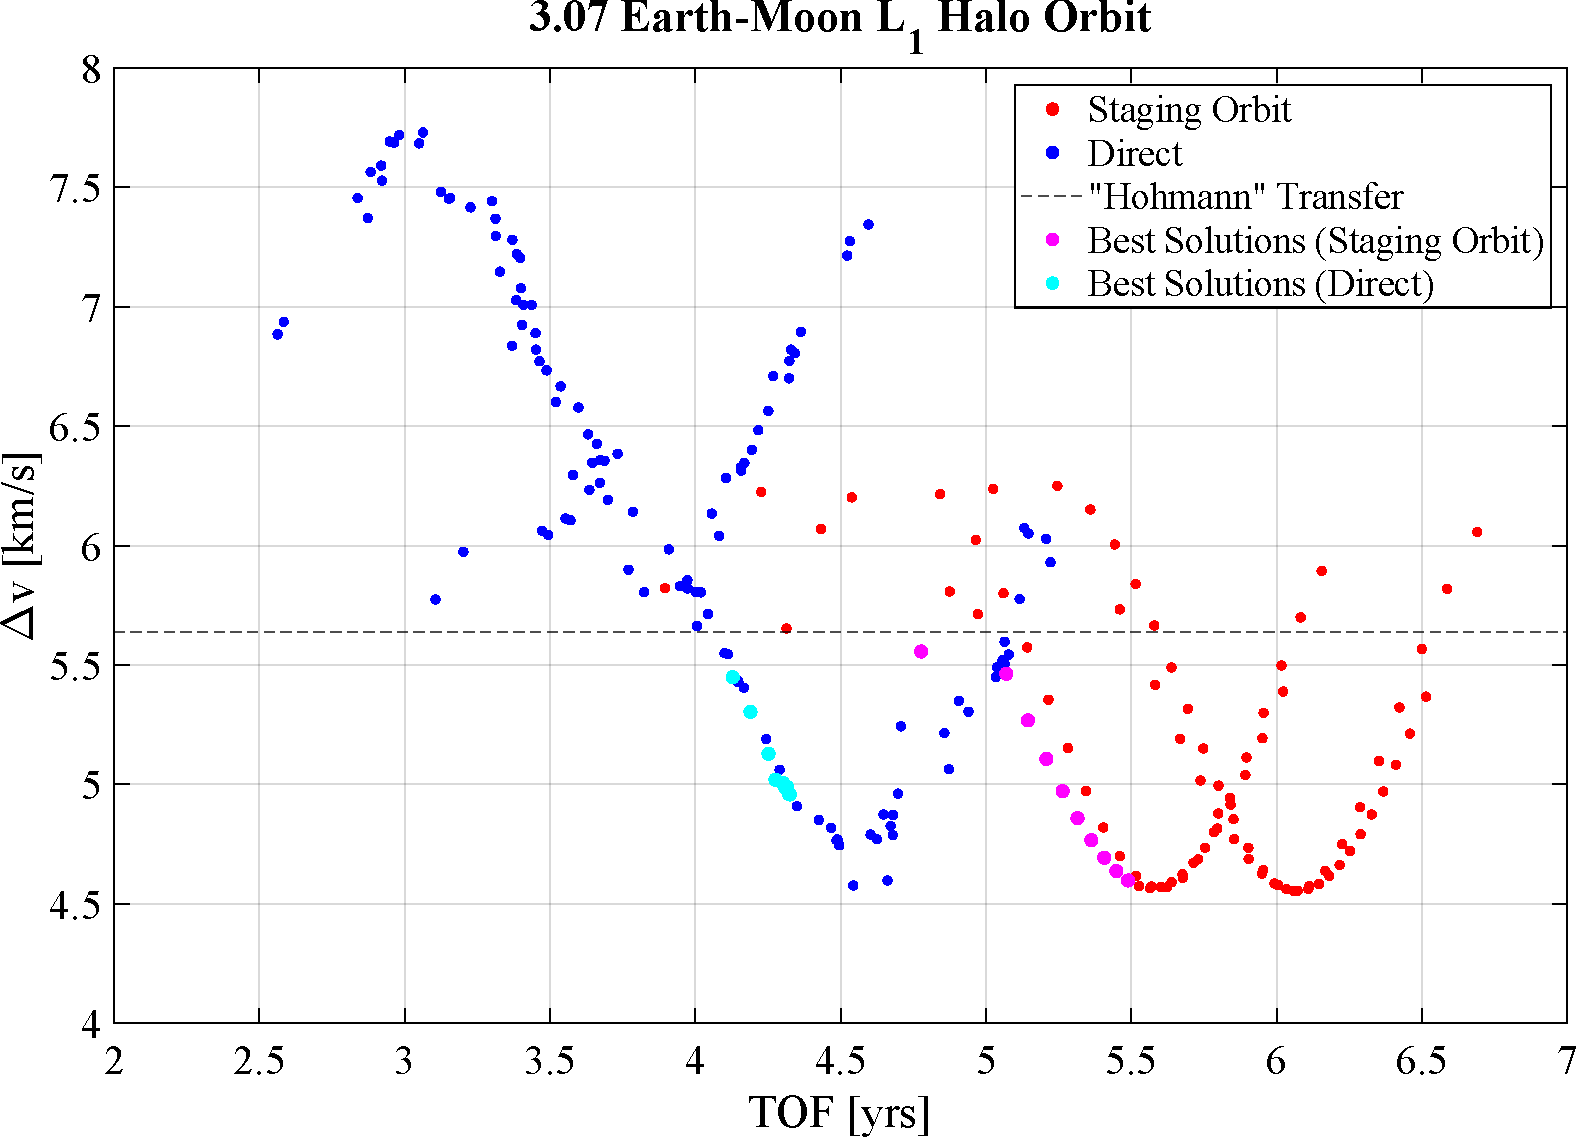
\includegraphics[width=0.75\textwidth]{figures/TradeSpace_L1Halo_3_07.pdf}
    \caption{Transfer tradespace departing from an Earth-Moon $L_{1}$ northern halo orbit ($JC=3.07$).}
    \label{fig:lowDeltav}
\end{figure}

If total TOF and total maneuver $\Delta v$ are considered to have units of years and km/s,
respectively, then these values have similar orders of magnitude for these transfers. Therefore, an
appropriate cost function needs to place weights on the two parameters depending on desired
transfer characteristics that are mission-dependent:
\begin{equation}
    J=\alpha TOF+\beta\Delta v,
    \label{eq:costfunction}
\end{equation}
where $J$ is the cost function value and $\alpha$ and $\beta$ are design variables to adjust the
cost function. $\alpha$ and $\beta$ can be adjusted to put higher priority on TOF or $\Delta v$,
depending on the particular application. This investigation uses $\alpha=5$ and $\beta=2$ to
prioritize lower TOF while still looking for decreased maneuver costs. This cost function is
applied to the transfers in the tradespace that are below the "Hohmann" transfer $\Delta v$
baseline, and the ten transfers from each transfer category that have the lowest $J$-value are
determined to be the best transfers for this application. For the case of the $L_{1}$ halo with
$JC=3.07$ in \cref{fig:lowDeltav}, these are the cyan ("direct") and magenta ("staging") points.

\subsection{Comparison of Best Solutions}
In \cref{fig:lowDeltav}, among the best solutions selected using the cost function, the "direct"
options still have lower times-of-flight, while the transfers with staging orbits achieve lower
$\Delta v$ costs on average. This contrasts with the earlier example from \cref{fig:tradespace},
now shown with the best solutions from the cost function in \cref{fig:lowBoth}. Here the "direct"
options have both lower times-of-flight and maneuver costs when compared to the staging orbit
transfers. Other scenarios result in "direct" transfers that are less desirable than the staging
orbit transfers. \cref{fig:betterStaging} shows transfers departing from an $L_{2}$ Lyapunov orbit,
where the transfers that utilize a staging orbit perform better in general with regards to both TOF
and maneuver $\Delta v$.

\begin{figure}[ht]
    \centering
    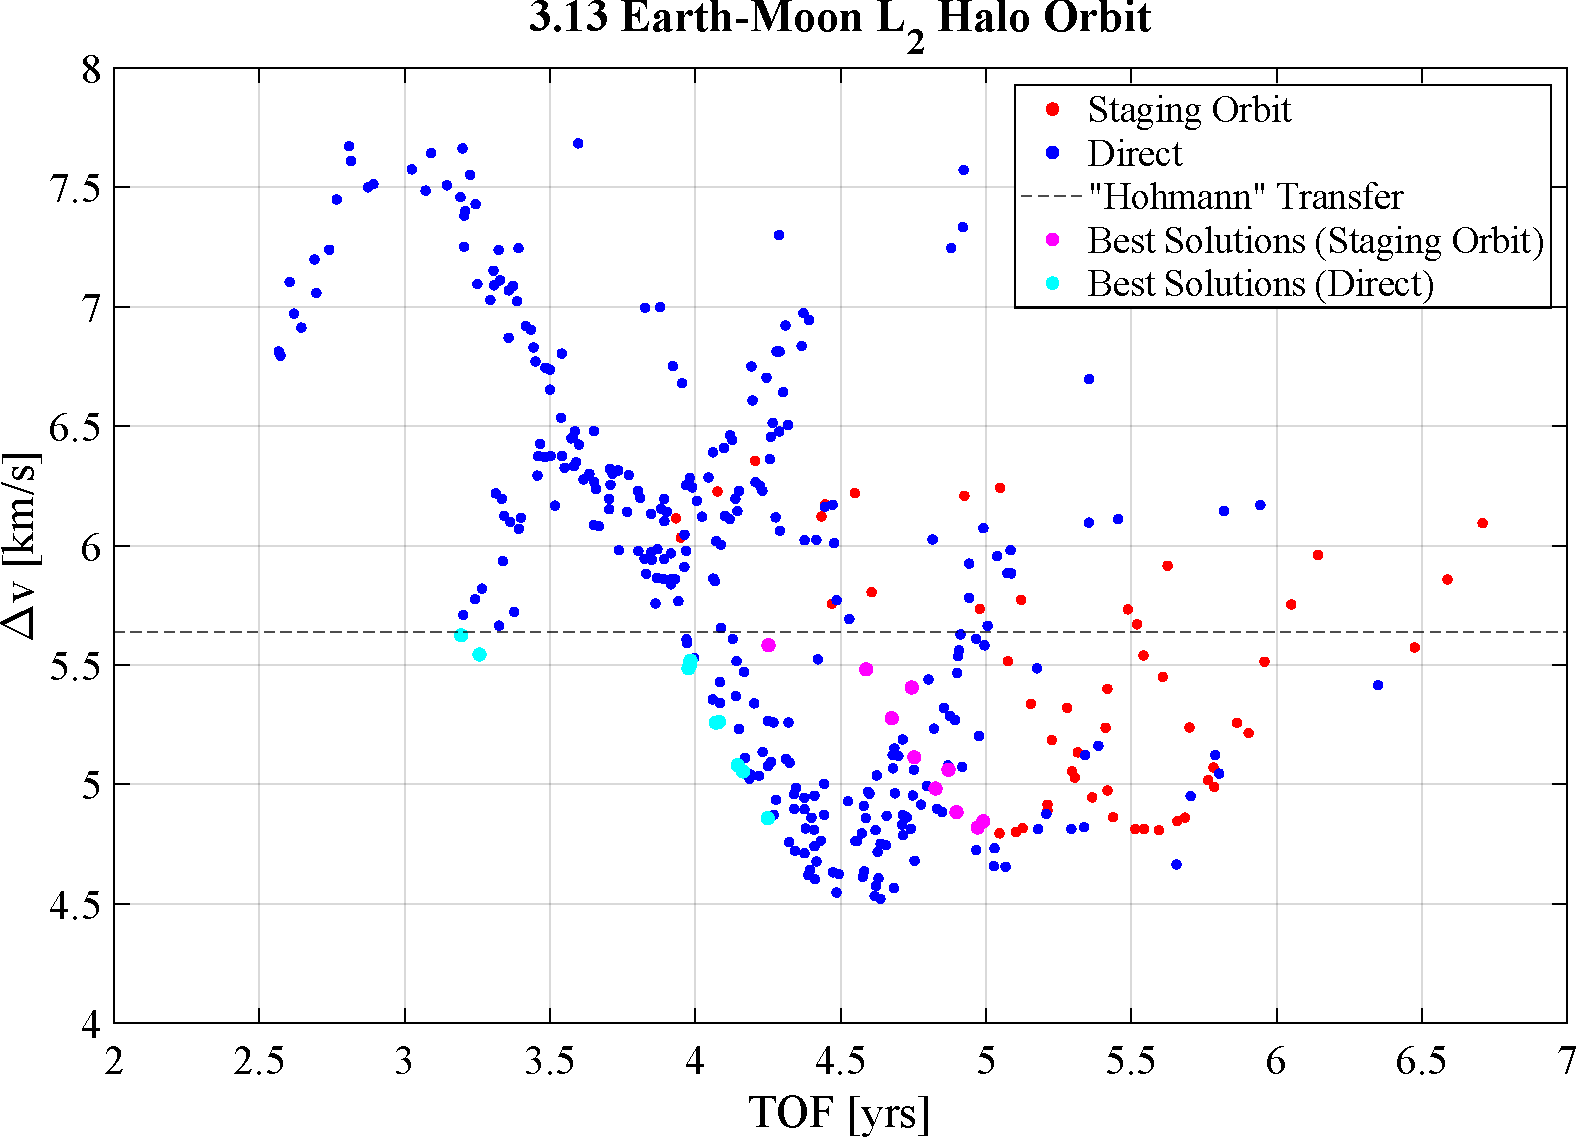
\includegraphics[width=0.75\textwidth]{figures/TradeSpace_L2Halo_3_13.pdf}
    \caption{Transfer tradespace departing from an Earth-Moon $L_{2}$ northern halo orbit ($JC=3.13$).}
    \label{fig:lowBoth}
\end{figure}

\begin{figure}[ht]
    \centering
    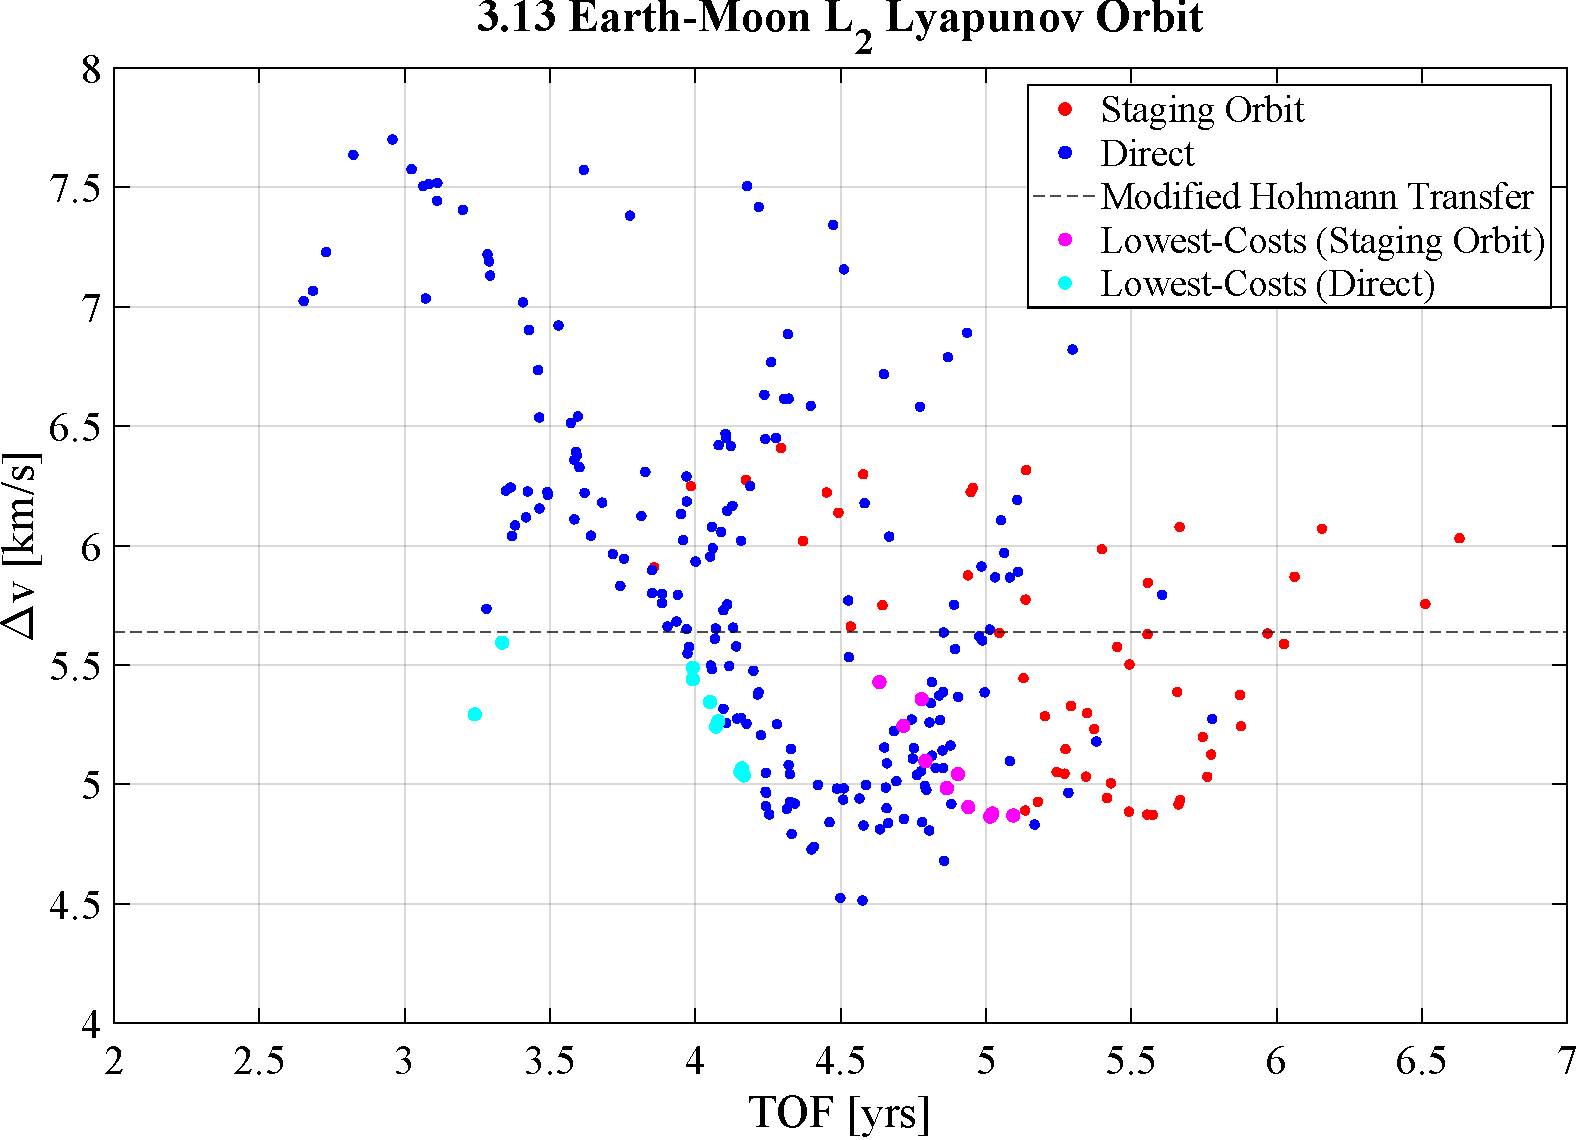
\includegraphics[width=0.75\textwidth]{figures/TradeSpace_L2Lyapunov_3_13.pdf}
    \caption{Transfer tradespace departing from an Earth-Moon $L_{2}$ Lyapunov orbit ($JC=3.13$).}
    \label{fig:betterStaging}
\end{figure}

...
